\documentclass[conference]{IEEEtran}
%\IEEEoverridecommandlockouts
% The preceding line is only needed to identify funding in the first footnote. If that is unneeded, please comment it out.
\usepackage{cite}
\usepackage{amsmath,amssymb,amsfonts}
\usepackage{algorithmic}
\usepackage{graphicx}
\usepackage{textcomp}
\usepackage{xcolor}

%\usepackage{longtable}
%\usepackage{supertabular}
\usepackage{xtab}%,afterpage}
\usepackage{multicol}
\usepackage{pbox}


\def\BibTeX{{\rm B\kern-.05em{\sc i\kern-.025em b}\kern-.08em
    T\kern-.1667em\lower.7ex\hbox{E}\kern-.125emX}}
    
\bibliographystyle{IEEEtran}

\begin{document}

\title{A Review on Intersection Management Systems and recent IoT Integrated Approaches
%\thanks{Identify applicable funding agency here. If none, delete this.}
}

\author{\IEEEauthorblockN{1\textsuperscript{st} Gustavo Velasco-Hernandez}
\IEEEauthorblockA{\textit{School of Electrical and Electronics Engineering} \\
\textit{Universidad del Valle}\\
Cali, Colombia \\
velasco.gustavo@correounivalle.edu.co}
\and
\IEEEauthorblockN{2\textsuperscript{nd} Eduardo Caicedo-Bravo}
\IEEEauthorblockA{\textit{School of Electrical and Electronics Engineering} \\
\textit{Universidad del Valle}\\
Cali, Colombia \\
eduardo.caicedo@correounivalle.edu.co}
}

\maketitle

\begin{abstract}
This document is a model and instructions for \LaTeX.
This and the IEEEtran.cls file define the components of your paper [title, text, heads, etc.]. *CRITICAL: Do Not Use Symbols, Special Characters, Footnotes, 
or Math in Paper Title or Abstract.
\end{abstract}

\IEEEpeerreviewmaketitle

\begin{IEEEkeywords}
component, formatting, style, styling, insert
\end{IEEEkeywords}

\section{Introduction}
This document is a model and instructions for \LaTeX.
Please observe the conference page limits. 

\section{Intersection Management Systems}

Intelligent Transportation Systems includes a wide range of applications and services transversal to many knowledge areas. For classifying those services, some taxonomies have been proposed like the ones presented in \cite[Ch.1]{Sussman2005} and \cite{Williams2008}. From described categories and classes, Advanced Traffic Management Systems have to be considered when an intelligent handling of traffic needs to be deployed.

One of the most desirable scenarios to improve efficiency and safety is an intersection. This because intersections are places where vehicles arrive from different directions at different velocities, increasing the chances for incidents and crashes. Choi \cite{Choi2010} states that 40\% of reported traffic accidents in the US, were intersection related. Also, in  \cite{CorporacionFondodePrevencionVial2010}, is reported that for Colombia in 2011, most of the accidents in the main cities were at intersections.

Different types of applications and systems are conceived to address these issues. Some tasks performed by those systems are intersection monitoring, vehicles detection, incident warning, collision avoidance, among others. A typical Intersection Management System is composed by three main components: Data source, that could be infrastructure sensors, like inductive loops, range sensors or cameras, and vehicle sensors and traveling data; decision system, which is the core of the whole system, is in charge of analyse and process information provided by infrastructure, vehicles and authorities in order to identify objects, recognise patterns, predict future incidents, control traffic and generate safe decisions and warnings alerts; and finally, is the presentation and displaying of the output of decision system, through infrastructure using dynamic signals, traffic light controlling, or using direct communication with drivers or vehicles through on-board visualisation/notification system. A block diagram of a generic IMS is presented in figure \ref{arch}

\begin{figure}[ht!]
\centering
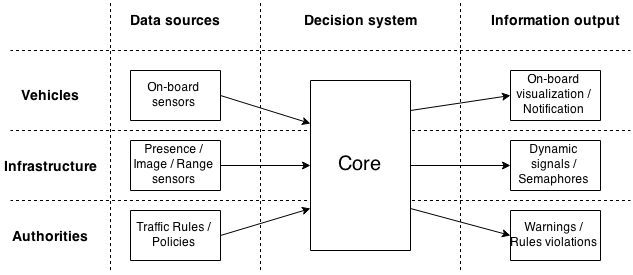
\includegraphics[scale=0.55]{fig/2/genericIMS.png}
\caption{Generic block diagram of an Intersection Management System.}
\label{arch}
\end{figure}

\subsection{Components in IMS application}

Intersection monitoring is a required task to be done within intelligent transportation systems for high-level applications like traffic analysis, counting and classification of vehicles or pedestrians, event prediction, incident detection and security and surveillance systems. Those applications have to take into account some of the elements depicted in figure \ref{arch} and developments in IMS have a wide range of approaches and objectives. In order to study IMS applications, five components have been defined, which are present on these applications, and on most cases, more than one component could be involved in the same development. In figure  \ref{imsComps} a graph is presented, showing aforementioned components and elements within them, and next, a description of each component is given.

\begin{figure}[ht!]
\centering
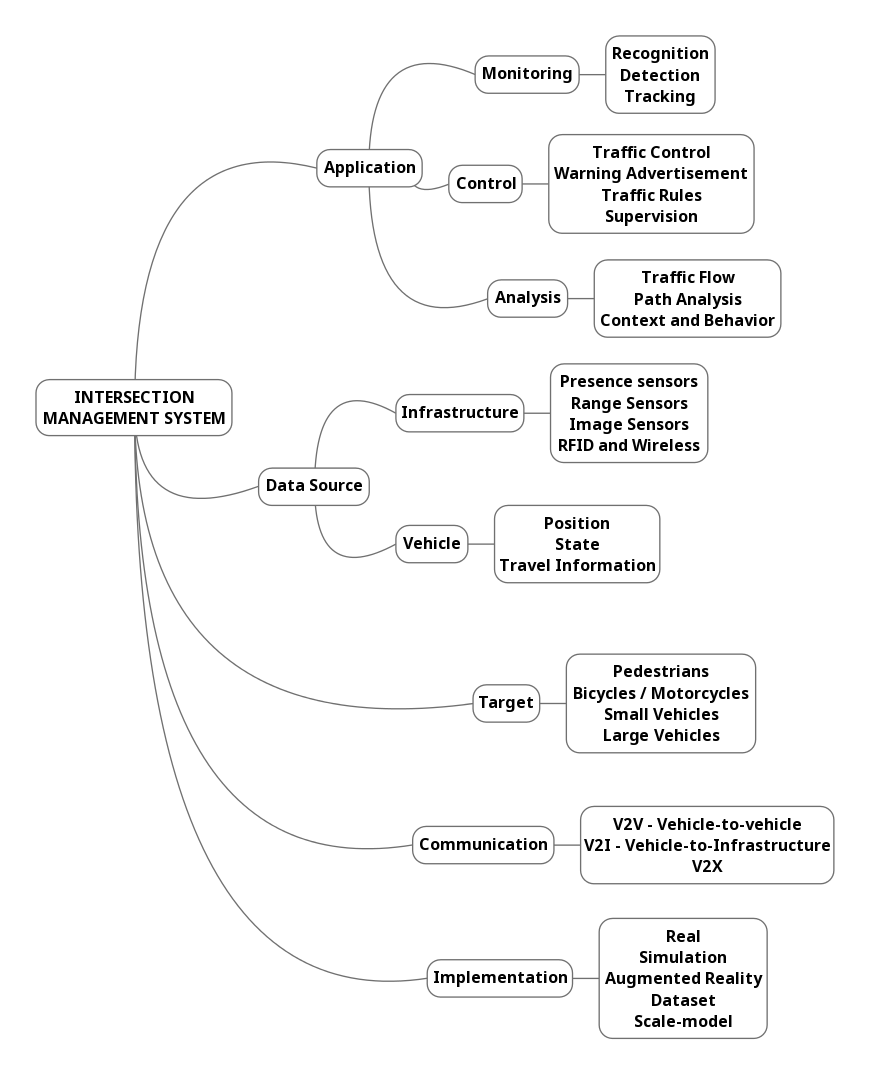
\includegraphics[scale=0.25]{fig/2/ims_graph5.png}
\caption{Components of an Intersection Management System application.}
\label{imsComps}
\end{figure}

\subsubsection{Application}

Application component could be seen as the final objective of the system. Generally, this includes high-level tasks like monitoring, analysis or control. Monitoring or surveillance systems execute actions like recognition, detection and/or tracking of objects in the scene. 
Other systems analyse the behaviour and interactions between detected objects to recognise path patterns, determine the context of the environment and predict some events of interest. At a higher level there are systems which make decisions based on detection of certain traffic conditions to handle traffic lights, control intersection access, generate warnings to drivers or issue traffic tickets when a rule violation exists.

\subsubsection{Data Source}

The origin of data is considered an independent component because of the variety of possible sources and posterior processing stages. From infrastructure side, data can be captured using a wide range of sensors like inductive loops, lasers, lidars and cameras. Also, monitoring connections to wireless networks. On the other side, data from vehicles is also useful for the system to enhance its representation of the scene and take decisions. This could be low-level data like vehicle state variables, for example, speed, orientation, acceleration, etc., or high-level data like travel information.


\subsubsection{Target}

In an intersection many objects of different kinds interact between them. Pedestrian and vehicles are found at intersections, and latter includes bicycles, motorcycles, cars, vans, buses, trucks and some other types of vehicles. For this reason some applications are designed for a specific element or group of elements. Pedestrian tracking, motorcycles recognition or car counting are examples of targeted applications.

\subsubsection{Communication}

One of the keypoints of ITS is how information technologies and communication advances are included in transportation. The main goal of this is to allow information sharing between vehicles and infrastructure entities. For this reason, 3 communication approaches appear: Vehicle-to-vehicle or Inter-vehicle communication (V2V), vehicle-to-infrastructure communication (V2I) and vehicle to both vehicle and infrastructure (V2X). Several protocols and standars have been proposed for these communication approaches, for example DSRC, WAVE and IEEE 802.11p, but research and development on this component is still active.

\subsubsection{Implementation}

Not all IMS applications are implementable on a real scenario, maybe because is not the scope of the application or because it is in a early stage and it could be validated in other ways. This types of developments are sometimes implemented and evaluated using simulators, making functional prototypes or deploying scale-models. Some other projects use datasets to evaluate new algorithms and data processing techniques, and then compare obtained results with previous works. Augmented reality is also used as a tool for evaluating and validate developments, taking advantage of the interaction of a real system with a simulated/artificial scenario.

\subsection{Developments in Intersection Management Systems}

In the table \ref{reviewtable} is presented a compilation of several developments within IMS field. For each work a brief comment is given, and a remark of how certain components (Data source, communication and application) are related to it. Target and implementation components could be infered from the comment.

%\clearpage 
%\onecolumn

% IMS review table
%\begin{center}
\footnotesize
%\begin{supertabular} {|c|p{0.3\linewidth}|p{0.15\linewidth}|p{0.1\linewidth}|c|}
%\begin{longtable} {|c|p{0.3\linewidth}|p{0.15\linewidth}|p{0.1\linewidth}|c|}
%\begin{xtabular*}{|c|p{0.3\linewidth}|p{0.15\linewidth}|p{0.1\linewidth}|c|}
%\begin{table}
%\afterpage{
%\onecolumn
\begin{table}
\onecolumn
\begin{xtabular*}{\textwidth}{|p{0.1\textwidth}|p{0.4\textwidth}|p{0.15\textwidth}|p{0.1\textwidth}|p{0.121875\linewidth}|}
%\begin{xtabular*}{\linewidth}{@{\extracolsep{\fill}}|*{5}{p{1.2cm}|}}
%\hline
%\multicolumn{5}{|c|}{ \textbf{Developments on Intersection Management Systems} } \\
%
%\hline
%\pbox{0.1\linewidth}{\textbf{Reference}} & 
%\pbox{0.4\linewidth}{\textbf{Comment}} & 
%\pbox{0.15\linewidth}{\textbf{Application}} & 
%\pbox{0.1\linewidth}{\textbf{Data Source}} & 
%\pbox{0.1\linewidth}{\textbf{Communication}} \\

\hline
%\endfirsthead
%\hline
%\textbf{Reference} & \textbf{Comment} & \textbf{Application} & \textbf{Data Source} & \textbf{Communication} \\
%\hline
%\endhead

%% IMS review table
\begin{center}
\footnotesize
\begin{longtable}{|c|p{0.3\linewidth}|p{0.15\linewidth}|p{0.1\linewidth}|c|}
%\begin{tabular}
\hline
\multicolumn{5}{|c|}{ \textbf{Developments on Intersection Management Systems} } \\

\hline
\textbf{Reference} & 
\pbox{0.3\linewidth}{\textbf{Comment}} & 
\pbox{0.15\linewidth}{\textbf{Application}} & 
\pbox{0.1\linewidth}{\textbf{Data Source}} & 
\textbf{Communication} \\

\hline
\endfirsthead
\hline
\textbf{Reference} & \textbf{Comment} & \textbf{Application} & \textbf{Data Source} & \textbf{Communication} \\
\hline
\endhead

\cite{Kamijo1999, Kamijo2000} & 
{They show an intersection monitoring system based on a fixed camera. This system is divided in three stages: Background modeling, object tracking and accident detection. They propose an innovative feature for accident detection using HMM.} & 
{Accident  detection} & 
Camera & 
N/A \\
\hline

\cite{Veeraraghavan2002} &
{Passive video-based system for monitoring an intersection. They implemented Stauffer's Method for background modeling, PCA for oriented bounding box computation, and Graph-based tracking and motion estimation. Also a simple methods for classification and calibration are described.} &
{Accident  detection} & 
Camera & 
N/A \\
\hline

%\cite{Gehrig2003} & & & & \\ \hline

\cite{Veeraraghavan2003} &
They present 4 stages for IMS: background modeling, motion tracking, feature extraction, calibration. They propose a 2-level tracking: Blob tracking as low-level and position using Kalman filter as high-level. &
Accident detection / prediction &
Camera & 
N/A \\
\hline

\cite{Messelodi2004} &
A Full implementation of an IMS in a town in northern Italy. The system claims to be independent of intersection geometry and it is based on a monocular camera. Processing stages of the system and classification approaches are described. &
Intersection Monitoring &
Camera &
N/A \\
\hline

\cite{Dogan2004} &
Development of a simulator for an Intersection Collision Warning System. Physical and MAC layers were modeled &
Intersection collision warning simulator &
N/A &
V2V \\
\hline

\cite{Chan2004} &
 Traffic monitoring for two context: Left-Turn-Across-Path-Opposite-Direction and Dilemma zone and red light violation &
Intersection Monitoring &
Radar &
N/A \\
\hline

\cite{Atev2005} &
A collision prediction system based on computational geometry is presented. The two main stages are low-level vision system for foreground optimization, with shaking compensation and noise removal, and a collision prediction system based on bounding boxes instead of bounding rectangles. &
Collision prediction &
Camera &
N/A \\
\hline

\cite{Chan2005} &
Analysis of Left-Turn-Across-Path-Opossite-Direction conflict situation. &
Intersection Monitoring &
Radar; Steering, speed sensors and GPS on-board &
V2X \\
\hline

\cite{Avila2005} &
Based on \cite{Dogan2004}, this works includes and improvement, including network layer and driver behaviour model. &
Intersection Simulator Architecture &
N/A &
V2X \\
\hline

\cite{Veeraraghavan2005} &
Tracking system based on Kalman filter for tracking and event detection at intersections, capable of detect 4 events: Acceleration, uniform velocity, stop and turns. &
Tracking and event detection &
Camera &
N/A \\
\hline

\cite{Zhao2006} &
Object tracking and classification at intersection using a single laser scanner. The system identifies 3 classes: Pedestrians, 2-wheeled vehicle and cars. It is based on points clustering, KL transform and markov chains &
Object tracking and classification &
Laser &
N/A \\
\hline

\cite{Eguchi2007} &
A system for discriminate an approaching vehicle to an intersection is described. It use a monocular camera and define a number of features for classification. Motion vectors are used too and determine the level of approaching. &
Vehicle detection &
Camera &
N/A \\
\hline

\cite{Kuramoto2007} &
A communication scheme based on nearest to intersection is described. Two zones are defined: nearest zone and quasi-nearest zone. Based on which zone vehicles are, communicaton is performed. Validation of proposal is done using a custom microscopic simulator. &
Intersection Communication Scheme &
N/A &
V2I \\
\hline

\cite{Dresner2008} &
A multiagent-based intersection control protocol called autonomous intersection management (AIM) is proposed. Based on a custom simulation, vehicles are modeled and they comunicate with an intersection manager which allows or deny access to intersection. It is possible to set different traffic policies, even for emulate current control approaches lke stop lights and traffic lights. &
Intersection Management &
On-board state sensors &
V2I \\
\hline

\cite{Jarupan2008} &
Based on \cite{Dogan2004} and \cite{Avila2005}, this simulator architecture emphasize on wireless communications. Now the system allows to compare different communication protocols and traffic configurations. &
Intersection Simulator Architecture &
N/A &
V2V \\
\hline

\cite{Zhao2008} &
Based on \cite{Zhao2006}, the system now includes more laser sensor for get a better representation of the scene, solving some occlusion issues. Clustering is used for grouping readings from different sensors belonging to the same object and a tracking approach based on angle of beam, range and time is presented. &
Intersection monitoring &
Lasers &
N/A \\
\hline

\cite{Rawashdeh2008} &
Proposal of a communication architecture for vehicles approaching to an intersection. Two zones are defined: Control Channel Zone (CCHZ) and Service Channel Zone (SCHZ). Also, 3 different methods are described for the system to be implmented &
Collision avoidance &
N/A &
V2I \\
\hline

\cite{Mundewadikar2008} &
Proposal of a physical-layer protocol for V2I communication at intersections. The system is evaluated in simulation using MATLAB &
Collision detection and warning &
N/A &
V2I \\
\hline

\cite{Zhao2009} &
Based on \cite{Zhao2008}, now the system includes a camera for video capture. In this video, data obtained from the lasers-based system are projected, drawing bounding boxes for vehicles and lines for trajectories. &
Intersection monitoring &
Camera, Lasers &
N/A \\
\hline

\cite{Abbas2009} &
Monitoring dilemma zone and efectiveness of control policies using cameras and loop detectors on an intersection &
Intersection monitoring &
Cameras, loop detectors &
N/A \\
\hline

\cite{Babaei2010} &
Author presents a system for foreground extraction, vehicle detection and tracking. A novel algorithm is proposed based on image division in traffic zones to perform background removal and vehicle detection. This proposal is compared with traditional MoG approach. &
Intersection monitoring &
Camera &
N/A \\
\hline

\cite{Meissner2010} &
A semi-automatic calibration method for a network of lidar sensors is presented using a custom simulation environment. Also, a calibration object were designed based on simulation results. &
Intersection Monitoring &
Lidars &
N/A \\
\hline

\cite{Quinlan2010} &
An augmented reality implementation of the system proposed in cite{Dresner2008} is presented. In this work, an autonomous vehicle is deployed in a mixed-reality platform and request to an virtual intersection manager for authorisation to cross and is the manager which decides if it is safe to cross or not, depending on the defined traffic policies and the state of virtual vehicles. &
Intersection management &
On-board state sensors &
V2I \\
\hline

\cite{Ball2010} &
The use of intelligent objects in vehicles is proposed. With sharing vehicle state information and jouney plans, the system aims to better control traffic in intersection using a novel back-off protocol instead of time traffic control system. &
Traffic control &
On-board state sensors, Journey plans &
V2V \\
\hline

\cite{Babaei2011} &
A system for traffic flow measurement based on anormalities detection is presented. Multiple cameras are used SIFT and unsupervised SVM-based clustering are performed for trajectories analysis. &
Intersection monitoring &
Cameras &
N/A \\
\hline

\cite{Basma2011} &
In presented system, wireless magnetic nodes are used to detect presence and to send data to a base station, which determines possible collisions and warns driver through a visualisation system in infrastructure. &
Collision Avoidance	 &
Presence sensors &
N/A \\
\hline

\cite{Azimi2012} &
An intersection control protocol based on V2V communication is proposed. This protocol is in charge of handling other vehicles messages and determines if is it safe or not to cross. They present two policies for managing intersection access: Concurrent Crossing- Intersection Protocol (CC-IP) and Maximum Progression-Intersection Protocol (MP-IP). &
Intersection management &
N/A &
V2V \\
\hline

\cite{CondeBento2012} &
A microscopic simulator was developed, with a spatial-temporal-based approach for managing the intersection. It is possible to implement different traffic policies for comparison purposes and the system works on crossroads and roundabouts. &
Intersection management &
On-board state sensors &
V2X \\
\hline

\cite{Zhao2012} &
A novel approach for detecting moving objects and track them is presented. The focus of this work relies on process merged data from laser sensors (\cite{Zhao2009}) to get better results at tracking. &
Object detection and tracking &
Lasers &
N/A \\
\hline

\cite{Jin2012} &
A Multiagent-based system is proposed. They define a Vehicle Agent and and Intersection Agent and propose a protocol for controlling intersection access based on timeslots, Also, the present a vehicle motion planning algorithm. Validation and testing was done using SUMO platform &
Intersection Management &
On-board state sensors &
V2I \\
\hline

\cite{Meissner2012} &
A set of laser scanners is used for detect and track pedestrians. GMM and DBSCAN are proposed for detection stage. For tracking purpose, a random finite set particle filter is used. &
Pedestrians detection and tracking &
Lasers &
N/A \\
\hline

\cite{Goldhammer2012} &
In this work is presented the setting and configuration of a multisensor network, based on 14 lasers, 10 cameras, GPS and V2I unit. Calibration and spatial-temporal alignment is performed. &
System Architecture &
Cameras, Lasers &
V2I \\
\hline

\cite{Friesen2013} &
A set of wireless probes are deployed to estimate traffic flow based on bluetooth connections. Then, using Zigbee, data is send to a master node which handle data for forwarding to a server / database for further processing. &
Traffic monitoring &
Wireless sensor network &
N/A \\
\hline

\cite{Guerrero-Ibanez2013} &
Two modes of Intersection Access Control: V2I mode and V2V mode. Implementation was done using minirobots in a scale model of an intersection. &
Intersection access control &
Loop detectors and RFID nodes &
V2X \\
\hline

%\cite{Meissner2013,Meissner2013a} &
% &
% &
% &
% \\
%\hline

\cite{Meissner2013b} &
A new method for object detection based on lidars data is proposed. After perform background removal, they use DBGridSCAN for 3D clustering and 2D pathway tracking. Then a combination of 2D-3D is done. The proposal is validated using OSPA metric. &
Object Detection &
Lasers &
N/A \\
\hline

\cite{Au2015} &
On top of AIM (\cite{Dresner2008}) Semi-AIM protocol is proposed. Assuming that human-driven vehicles to autonomous vehicles transition will be long, this system is intended for semi-autonomous vehicles. Also the author describe the human relation to a semi-autonomous vehicle and analyse how the features of autonomy employed by the car affects the traffic delay. &
Intersection Management &
On-board state sensors &
V2I \\
\hline

%\cite{} &
% &
% &
% &
% \\
%\hline

%\cite{} &
% &
% &
% &
% \\
%\hline

%\cite{} &
% &
% &
% &
% \\
%\hline

%\cite{} &
% &
% &
% &
% \\
%\hline

%\cite{} &
% &
% &
% &
% \\
%\hline

%\cite{} &
% &
% &
% &
% \\
%\hline


\hline
%\end{tabular}
\caption{Developments related to Intersection Management Systems.}
\label{reviewtable}
\end{longtable}
\end{center}

%\begin{table*}[tp]
%\caption{Developments on Intersection Management Systems}
%\label{reviewtable}
%\begin{xtabular*}{\textwidth}{|p{0.08\textwidth}|p{0.41\textwidth}|p{0.15\textwidth}|p{0.12\textwidth}|p{0.121875\linewidth}|}
%
%\hline
%\textbf{Reference} & \textbf{Comment} & \textbf{Application} & \textbf{Data Source} & \textbf{Communication} \\
%\hline
%
%
%\cite{Kamijo1999, Kamijo2000} & 
%{They show an intersection monitoring system based on a fixed camera. This system is divided in three stages: Background modeling, object tracking and accident detection. They propose an innovative feature for accident detection using HMM.} & 
%{Accident  detection} & 
%Camera & 
%N/A \\
%\hline
%
%\cite{Veeraraghavan2002} &
%{Passive video-based system for monitoring an intersection. They implemented Stauffer's Method for background modeling, PCA for oriented bounding box computation, and Graph-based tracking and motion estimation. Also a simple methods for classification and calibration are described.} &
%{Accident  detection} & 
%Camera & 
%N/A \\
%\hline
%
%%\cite{Gehrig2003} & & & & \\ \hline
%
%\cite{Veeraraghavan2003} &
%They present 4 stages for IMS: background modeling, motion tracking, feature extraction, calibration. They propose a 2-level tracking: Blob tracking as low-level and position using Kalman filter as high-level. &
%Accident detection / prediction &
%Camera & 
%N/A \\
%\hline
%
%\cite{Messelodi2004} &
%A Full implementation of an IMS in a town in northern Italy. The system claims to be independent of intersection geometry and it is based on a monocular camera. Processing stages of the system and classification approaches are described. &
%Intersection Monitoring &
%Camera &
%N/A \\
%\hline
%
%\cite{Dogan2004} &
%Development of a simulator for an Intersection Collision Warning System. Physical and MAC layers were modeled &
%Intersection collision warning simulator &
%N/A &
%V2V \\
%\hline
%
%\cite{Chan2004} &
% Traffic monitoring for two context: Left-Turn-Across-Path-Opposite-Direction and Dilemma zone and red light violation &
%Intersection Monitoring &
%Radar &
%N/A \\
%\hline
%
%\cite{Atev2005} &
%A collision prediction system based on computational geometry is presented. The two main stages are low-level vision system for foreground optimization, with shaking compensation and noise removal, and a collision prediction system based on bounding boxes instead of bounding rectangles. &
%Collision prediction &
%Camera &
%N/A \\
%\hline
%
%\cite{Chan2005} &
%Analysis of Left-Turn-Across-Path-Opossite-Direction conflict situation. &
%Intersection Monitoring &
%Radar; Steering, speed sensors and GPS on-board &
%V2X \\
%\hline
%
%\cite{Avila2005} &
%Based on \cite{Dogan2004}, this works includes and improvement, including network layer and driver behaviour model. &
%Intersection Simulator Architecture &
%N/A &
%V2X \\
%\hline
%
%\cite{Veeraraghavan2005} &
%Tracking system based on Kalman filter for tracking and event detection at intersections, capable of detect 4 events: Acceleration, uniform velocity, stop and turns. &
%Tracking and event detection &
%Camera &
%N/A \\
%\hline
%
%\cite{Zhao2006} &
%Object tracking and classification at intersection using a single laser scanner. The system identifies 3 classes: Pedestrians, 2-wheeled vehicle and cars. It is based on points clustering, KL transform and markov chains &
%Object tracking and classification &
%Laser &
%N/A \\
%\hline
%
%\cite{Eguchi2007} &
%A system for discriminate an approaching vehicle to an intersection is described. It use a monocular camera and define a number of features for classification. Motion vectors are used too and determine the level of approaching. &
%Vehicle detection &
%Camera &
%N/A \\
%\hline
%
%\cite{Kuramoto2007} &
%A communication scheme based on nearest to intersection is described. Two zones are defined: nearest zone and quasi-nearest zone. Based on which zone vehicles are, communicaton is performed. Validation of proposal is done using a custom microscopic simulator. &
%Intersection Communication Scheme &
%N/A &
%V2I \\
%\hline
%
%\cite{Dresner2008} &
%A multiagent-based intersection control protocol called autonomous intersection management (AIM) is proposed. Based on a custom simulation, vehicles are modeled and they comunicate with an intersection manager which allows or deny access to intersection. It is possible to set different traffic policies, even for emulate current control approaches lke stop lights and traffic lights. &
%Intersection Management &
%On-board state sensors &
%V2I \\
%\hline
%
%\cite{Jarupan2008} &
%Based on \cite{Dogan2004} and \cite{Avila2005}, this simulator architecture emphasize on wireless communications. Now the system allows to compare different communication protocols and traffic configurations. &
%Intersection Simulator Architecture &
%N/A &
%V2V \\
%\hline
%
%\cite{Zhao2008} &
%Based on \cite{Zhao2006}, the system now includes more laser sensor for get a better representation of the scene, solving some occlusion issues. Clustering is used for grouping readings from different sensors belonging to the same object and a tracking approach based on angle of beam, range and time is presented. &
%Intersection monitoring &
%Lasers &
%N/A \\
%\hline
%
%\cite{Rawashdeh2008} &
%Proposal of a communication architecture for vehicles approaching to an intersection. Two zones are defined: Control Channel Zone (CCHZ) and Service Channel Zone (SCHZ). Also, 3 different methods are described for the system to be implmented &
%Collision avoidance &
%N/A &
%V2I \\
%\hline
%
%\cite{Mundewadikar2008} &
%Proposal of a physical-layer protocol for V2I communication at intersections. The system is evaluated in simulation using MATLAB &
%Collision detection and warning &
%N/A &
%V2I \\
%\hline
%
%\cite{Zhao2009} &
%Based on \cite{Zhao2008}, now the system includes a camera for video capture. In this video, data obtained from the lasers-based system are projected, drawing bounding boxes for vehicles and lines for trajectories. &
%Intersection monitoring &
%Camera, Lasers &
%N/A \\
%\hline
%
%\end{xtabular*}
%\end{table*}

%\begin{table*}[tp]
%\caption{Developments on Intersection Management Systems}
%\label{reviewtable}
%\begin{xtabular*}{\textwidth}{|p{0.08\textwidth}|p{0.41\textwidth}|p{0.15\textwidth}|p{0.12\textwidth}|p{0.121875\linewidth}|}
%
%\hline
%\textbf{Reference} & \textbf{Comment} & \textbf{Application} & \textbf{Data Source} & \textbf{Communication} \\
%\hline
%
%
%\cite{Abbas2009} &
%Monitoring dilemma zone and efectiveness of control policies using cameras and loop detectors on an intersection &
%Intersection monitoring &
%Cameras, loop detectors &
%N/A \\
%\hline
%
%
%\cite{Babaei2010} &
%Author presents a system for foreground extraction, vehicle detection and tracking. A novel algorithm is proposed based on image division in traffic zones to perform background removal and vehicle detection. This proposal is compared with traditional MoG approach. &
%Intersection monitoring &
%Camera &
%N/A \\
%\hline
%
%\cite{Meissner2010} &
%A semi-automatic calibration method for a network of lidar sensors is presented using a custom simulation environment. Also, a calibration object were designed based on simulation results. &
%Intersection Monitoring &
%Lidars &
%N/A \\
%\hline

\begin{table*}[tp]
\footnotesize
\caption{Developments on Intersection Management Systems}
\label{reviewtable}
\begin{xtabular*}{\textwidth}{|p{0.08\textwidth}|p{0.45\textwidth}|p{0.11\textwidth}|p{0.12\textwidth}|p{0.121875\linewidth}|}

\hline
\textbf{Reference} & \textbf{Comment} & \textbf{Application} & \textbf{Data Source} & \textbf{Communication} \\
\hline

%\cite{Quinlan2010} &
%An augmented reality implementation of the system proposed in cite{Dresner2008} is presented. In this work, an autonomous vehicle is deployed in a mixed-reality platform and request to an virtual intersection manager for authorisation to cross and is the manager which decides if it is safe to cross or not, depending on the defined traffic policies and the state of virtual vehicles. &
%Intersection management &
%On-board state sensors &
%V2I \\
%\hline

%\cite{Ball2010} &
%The use of intelligent objects in vehicles is proposed. With sharing vehicle state information and jouney plans, the system aims to better control traffic in intersection using a novel back-off protocol instead of time traffic control system. &
%Traffic control &
%On-board state sensors, Journey plans &
%V2V \\
%\hline

\cite{Babaei2011} &
A system for traffic flow measurement based on anormalities detection is presented. Multiple cameras are used SIFT and unsupervised SVM-based clustering are performed for trajectories analysis. &
Intersection monitoring &
Cameras &
N/A \\
\hline

\cite{Basma2011} &
In presented system, wireless magnetic nodes are used to detect presence and to send data to a base station, which determines possible collisions and warns driver through a visualisation system in infrastructure. &
Collision Avoidance	 &
Presence sensors &
N/A \\
\hline

\cite{Azimi2012} &
An intersection control protocol based on V2V communication is proposed. This protocol is in charge of handling other vehicles messages and determines if is it safe or not to cross. They present two policies for managing intersection access: Concurrent Crossing- Intersection Protocol (CC-IP) and Maximum Progression-Intersection Protocol (MP-IP). &
Intersection management &
N/A &
V2V \\
\hline

\cite{CondeBento2012} &
A microscopic simulator was developed, with a spatial-temporal-based approach for managing the intersection. It is possible to implement different traffic policies for comparison purposes and the system works on crossroads and roundabouts. &
Intersection management &
On-board state sensors &
V2X \\
\hline

\cite{Zhao2012} &
A novel approach for detecting moving objects and track them is presented. The focus of this work relies on process merged data from laser sensors (\cite{Zhao2009}) to get better results at tracking. &
Object detection and tracking &
Lasers &
N/A \\
\hline

\cite{Jin2012} &
A Multiagent-based system is proposed. They define a Vehicle Agent and and Intersection Agent and propose a protocol for controlling intersection access based on timeslots, Also, the present a vehicle motion planning algorithm. Validation and testing was done using SUMO platform &
Intersection Management &
On-board state sensors &
V2I \\
\hline

\cite{Meissner2012} &
A set of laser scanners is used for detect and track pedestrians. GMM and DBSCAN are proposed for detection stage. For tracking purpose, a random finite set particle filter is used. &
Pedestrians detection and tracking &
Lasers &
N/A \\
\hline

\cite{Goldhammer2012} &
In this work is presented the setting and configuration of a multisensor network, based on 14 lasers, 10 cameras, GPS and V2I unit. Calibration and spatial-temporal alignment is performed. &
System Architecture &
Cameras, Lasers &
V2I \\
\hline

\cite{Friesen2013} &
A set of wireless probes are deployed to estimate traffic flow based on bluetooth connections. Then, using Zigbee, data is send to a master node which handle data for forwarding to a server / database for further processing. &
Traffic monitoring &
Wireless sensor network &
N/A \\
\hline

\cite{Guerrero-Ibanez2013} &
Two modes of Intersection Access Control: V2I mode and V2V mode. Implementation was done using minirobots in a scale model of an intersection. &
Intersection access control &
Loop detectors and RFID nodes &
V2X \\
\hline

%\cite{Meissner2013,Meissner2013a} &
% &
% &
% &
% \\
%\hline

\cite{Meissner2013b} &
A new method for object detection based on lidars data is proposed. After perform background removal, they use DBGridSCAN for 3D clustering and 2D pathway tracking. Then a combination of 2D-3D is done. The proposal is validated using OSPA metric. &
Object Detection &
Lasers &
N/A \\
\hline

\cite{Au2015} &
On top of AIM (\cite{Dresner2008}) Semi-AIM protocol is proposed. Assuming that human-driven vehicles to autonomous vehicles transition will be long, this system is intended for semi-autonomous vehicles. Also the author describe the human relation to a semi-autonomous vehicle and analyse how the features of autonomy employed by the car affects the traffic delay. &
Intersection Management &
On-board state sensors &
V2I \\
\hline

\end{xtabular*}
\twocolumn
%} % end of scope of "\afterpage" directive
%\caption{Developments related to Intersection Management Systems.}
\label{reviewtable}
%\end{table}
%\end{longtable}
%\end{supertabular}
%\end{center}
\end{table}



%\twocolumn




\section{Ease of Use}

\subsection{Maintaining the Integrity of the Specifications}

The IEEEtran class file is used to format your paper and style the text. All margins, 
column widths, line spaces, and text fonts are prescribed; please do not 
alter them. You may note peculiarities. For example, the head margin
measures proportionately more than is customary. This measurement 
and others are deliberate, using specifications that anticipate your paper 
as one part of the entire proceedings, and not as an independent document. 
Please do not revise any of the current designations.

\section{Prepare Your Paper Before Styling}
Before you begin to format your paper, first write and save the content as a 
separate text file. Complete all content and organizational editing before 
formatting. Please note sections \ref{AA}--\ref{SCM} below for more information on 
proofreading, spelling and grammar.

Keep your text and graphic files separate until after the text has been 
formatted and styled. Do not number text heads---{\LaTeX} will do that 
for you.


\begin {table}[htb]
\begin{tabular*}{\textwidth}{@{\hskip 6pt\extracolsep{\stretch{1}}}*{9}{r}}
\hline
M       & TA    & MO    & P & N & ID & CC & XC & KL \\
\hline
method  & 0.79  & 0.59  & - & - & 4  & 3  & 5  &    \\
ED  []  & 5     & 7     & - & - & 6  &    &    &    \\
CR      & 4     & 7     & - & - & 22 &    &    &    \\
NB[]    & 2     & 75    & - & - & 6  &    &    &    \\
\hline
\end{tabular*}
\caption{Set of observations }
\end{table}

\subsection{Abbreviations and Acronyms}\label{AA}
Define abbreviations and acronyms the first time they are used in the text, 
even after they have been defined in the abstract. Abbreviations such as 
IEEE, SI, MKS, CGS, ac, dc, and rms do not have to be defined. Do not use 
abbreviations in the title or heads unless they are unavoidable.

\subsection{Units}
\begin{itemize}
\item Use either SI (MKS) or CGS as primary units. (SI units are encouraged.) English units may be used as secondary units (in parentheses). An exception would be the use of English units as identifiers in trade, such as ``3.5-inch disk drive''.
\item Avoid combining SI and CGS units, such as current in amperes and magnetic field in oersteds. This often leads to confusion because equations do not balance dimensionally. If you must use mixed units, clearly state the units for each quantity that you use in an equation.
\item Do not mix complete spellings and abbreviations of units: ``Wb/m\textsuperscript{2}'' or ``webers per square meter'', not ``webers/m\textsuperscript{2}''. Spell out units when they appear in text: ``. . . a few henries'', not ``. . . a few H''.
\item Use a zero before decimal points: ``0.25'', not ``.25''. Use ``cm\textsuperscript{3}'', not ``cc''.)
\end{itemize}

\subsection{Equations}
Number equations consecutively. To make your 
equations more compact, you may use the solidus (~/~), the exp function, or 
appropriate exponents. Italicize Roman symbols for quantities and variables, 
but not Greek symbols. Use a long dash rather than a hyphen for a minus 
sign. Punctuate equations with commas or periods when they are part of a 
sentence, as in:
\begin{equation}
a+b=\gamma\label{eq}
\end{equation}

Be sure that the 
symbols in your equation have been defined before or immediately following 
the equation. Use ``\eqref{eq}'', not ``Eq.~\eqref{eq}'' or ``equation \eqref{eq}'', except at 
the beginning of a sentence: ``Equation \eqref{eq} is . . .''

\subsection{\LaTeX-Specific Advice}

Please use ``soft'' (e.g., \verb|\eqref{Eq}|) cross references instead
of ``hard'' references (e.g., \verb|(1)|). That will make it possible
to combine sections, add equations, or change the order of figures or
citations without having to go through the file line by line.

Please don't use the \verb|{eqnarray}| equation environment. Use
\verb|{align}| or \verb|{IEEEeqnarray}| instead. The \verb|{eqnarray}|
environment leaves unsightly spaces around relation symbols.

Please note that the \verb|{subequations}| environment in {\LaTeX}
will increment the main equation counter even when there are no
equation numbers displayed. If you forget that, you might write an
article in which the equation numbers skip from (17) to (20), causing
the copy editors to wonder if you've discovered a new method of
counting.

{\BibTeX} does not work by magic. It doesn't get the bibliographic
data from thin air but from .bib files. If you use {\BibTeX} to produce a
bibliography you must send the .bib files. 

{\LaTeX} can't read your mind. If you assign the same label to a
subsubsection and a table, you might find that Table I has been cross
referenced as Table IV-B3. 

{\LaTeX} does not have precognitive abilities. If you put a
\verb|\label| command before the command that updates the counter it's
supposed to be using, the label will pick up the last counter to be
cross referenced instead. In particular, a \verb|\label| command
should not go before the caption of a figure or a table.

Do not use \verb|\nonumber| inside the \verb|{array}| environment. It
will not stop equation numbers inside \verb|{array}| (there won't be
any anyway) and it might stop a wanted equation number in the
surrounding equation.

\subsection{Some Common Mistakes}\label{SCM}
\begin{itemize}
\item The word ``data'' is plural, not singular.
\item The subscript for the permeability of vacuum $\mu_{0}$, and other common scientific constants, is zero with subscript formatting, not a lowercase letter ``o''.
\item In American English, commas, semicolons, periods, question and exclamation marks are located within quotation marks only when a complete thought or name is cited, such as a title or full quotation. When quotation marks are used, instead of a bold or italic typeface, to highlight a word or phrase, punctuation should appear outside of the quotation marks. A parenthetical phrase or statement at the end of a sentence is punctuated outside of the closing parenthesis (like this). (A parenthetical sentence is punctuated within the parentheses.)
\item A graph within a graph is an ``inset'', not an ``insert''. The word alternatively is preferred to the word ``alternately'' (unless you really mean something that alternates).
\item Do not use the word ``essentially'' to mean ``approximately'' or ``effectively''.
\item In your paper title, if the words ``that uses'' can accurately replace the word ``using'', capitalize the ``u''; if not, keep using lower-cased.
\item Be aware of the different meanings of the homophones ``affect'' and ``effect'', ``complement'' and ``compliment'', ``discreet'' and ``discrete'', ``principal'' and ``principle''.
\item Do not confuse ``imply'' and ``infer''.
\item The prefix ``non'' is not a word; it should be joined to the word it modifies, usually without a hyphen.
\item There is no period after the ``et'' in the Latin abbreviation ``et al.''.
\item The abbreviation ``i.e.'' means ``that is'', and the abbreviation ``e.g.'' means ``for example''.
\end{itemize}
An excellent style manual for science writers is \cite{b7}.

\subsection{Authors and Affiliations}
\textbf{The class file is designed for, but not limited to, six authors.} A 
minimum of one author is required for all conference articles. Author names 
should be listed starting from left to right and then moving down to the 
next line. This is the author sequence that will be used in future citations 
and by indexing services. Names should not be listed in columns nor group by 
affiliation. Please keep your affiliations as succinct as possible (for 
example, do not differentiate among departments of the same organization).

\subsection{Identify the Headings}
Headings, or heads, are organizational devices that guide the reader through 
your paper. There are two types: component heads and text heads.

Component heads identify the different components of your paper and are not 
topically subordinate to each other. Examples include Acknowledgments and 
References and, for these, the correct style to use is ``Heading 5''. Use 
``figure caption'' for your Figure captions, and ``table head'' for your 
table title. Run-in heads, such as ``Abstract'', will require you to apply a 
style (in this case, italic) in addition to the style provided by the drop 
down menu to differentiate the head from the text.

Text heads organize the topics on a relational, hierarchical basis. For 
example, the paper title is the primary text head because all subsequent 
material relates and elaborates on this one topic. If there are two or more 
sub-topics, the next level head (uppercase Roman numerals) should be used 
and, conversely, if there are not at least two sub-topics, then no subheads 
should be introduced.

\subsection{Figures and Tables}
\paragraph{Positioning Figures and Tables} Place figures and tables at the top and 
bottom of columns. Avoid placing them in the middle of columns. Large 
figures and tables may span across both columns. Figure captions should be 
below the figures; table heads should appear above the tables. Insert 
figures and tables after they are cited in the text. Use the abbreviation 
``Fig.~\ref{fig}'', even at the beginning of a sentence.

\begin{table}[htbp]
\caption{Table Type Styles}
\begin{center}
\begin{tabular}{|c|c|c|c|}
\hline
\textbf{Table}&\multicolumn{3}{|c|}{\textbf{Table Column Head}} \\
\cline{2-4} 
\textbf{Head} & \textbf{\textit{Table column subhead}}& \textbf{\textit{Subhead}}& \textbf{\textit{Subhead}} \\
\hline
copy& More table copy$^{\mathrm{a}}$& &  \\
\hline
\multicolumn{4}{l}{$^{\mathrm{a}}$Sample of a Table footnote.}
\end{tabular}
\label{tab1}
\end{center}
\end{table}

\begin{figure}[htbp]
\centerline{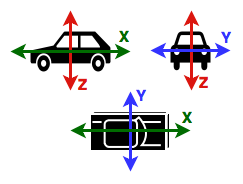
\includegraphics{fig1.png}}
\caption{Example of a figure caption.}
\label{fig}
\end{figure}

Figure Labels: Use 8 point Times New Roman for Figure labels. Use words 
rather than symbols or abbreviations when writing Figure axis labels to 
avoid confusing the reader. As an example, write the quantity 
``Magnetization'', or ``Magnetization, M'', not just ``M''. If including 
units in the label, present them within parentheses. Do not label axes only 
with units. In the example, write ``Magnetization (A/m)'' or ``Magnetization 
\{A[m(1)]\}'', not just ``A/m''. Do not label axes with a ratio of 
quantities and units. For example, write ``Temperature (K)'', not 
``Temperature/K''.

\section*{Acknowledgment}

The preferred spelling of the word ``acknowledgment'' in America is without 
an ``e'' after the ``g''. Avoid the stilted expression ``one of us (R. B. 
G.) thanks $\ldots$''. Instead, try ``R. B. G. thanks$\ldots$''. Put sponsor 
acknowledgments in the unnumbered footnote on the first page.

\section*{References}

Please number citations consecutively within brackets \cite{b1}. The 
sentence punctuation follows the bracket \cite{b2}. Refer simply to the reference 
number, as in \cite{b3}---do not use ``Ref. \cite{b3}'' or ``reference \cite{b3}'' except at 
the beginning of a sentence: ``Reference \cite{b3} was the first $\ldots$''

Number footnotes separately in superscripts. Place the actual footnote at 
the bottom of the column in which it was cited. Do not put footnotes in the 
abstract or reference list. Use letters for table footnotes.

Unless there are six authors or more give all authors' names; do not use 
``et al.''. Papers that have not been published, even if they have been 
submitted for publication, should be cited as ``unpublished'' \cite{b4}. Papers 
that have been accepted for publication should be cited as ``in press'' \cite{b5}. 
Capitalize only the first word in a paper title, except for proper nouns and 
element symbols.

For papers published in translation journals, please give the English 
citation first, followed by the original foreign-language citation \cite{b6}.

\bibliography{IEEEabrv,../bibliography}

\begin{thebibliography}{00}
\bibitem{b1} G. Eason, B. Noble, and I. N. Sneddon, ``On certain integrals of Lipschitz-Hankel type involving products of Bessel functions,'' Phil. Trans. Roy. Soc. London, vol. A247, pp. 529--551, April 1955.
\bibitem{b2} J. Clerk Maxwell, A Treatise on Electricity and Magnetism, 3rd ed., vol. 2. Oxford: Clarendon, 1892, pp.68--73.
\bibitem{b3} I. S. Jacobs and C. P. Bean, ``Fine particles, thin films and exchange anisotropy,'' in Magnetism, vol. III, G. T. Rado and H. Suhl, Eds. New York: Academic, 1963, pp. 271--350.
\bibitem{b4} K. Elissa, ``Title of paper if known,'' unpublished.
\bibitem{b5} R. Nicole, ``Title of paper with only first word capitalized,'' J. Name Stand. Abbrev., in press.
\bibitem{b6} Y. Yorozu, M. Hirano, K. Oka, and Y. Tagawa, ``Electron spectroscopy studies on magneto-optical media and plastic substrate interface,'' IEEE Transl. J. Magn. Japan, vol. 2, pp. 740--741, August 1987 [Digests 9th Annual Conf. Magnetics Japan, p. 301, 1982].
\bibitem{b7} M. Young, The Technical Writer's Handbook. Mill Valley, CA: University Science, 1989.
\end{thebibliography}
\vspace{12pt}
\color{red}
IEEE conference templates contain guidance text for composing and formatting conference papers. Please ensure that all template text is removed from your conference paper prior to submission to the conference. Failure to remove the template text from your paper may result in your paper not being published.

\end{document}
